\documentclass[a4paper]{article}

\usepackage{amsmath}
\usepackage{hyperref}
\usepackage{graphicx}
\usepackage{float}

\title{Using local binary patterns to read license plates in photographs}

% Paragraph indentation
\setlength{\parindent}{0pt}
\setlength{\parskip}{1ex plus 0.5ex minus 0.2ex}

\begin{document}
\maketitle

\section*{Project members}
Gijs van der Voort \\
Richard Torenvliet \\
Jayke Meijer \\
Tadde\"us Kroes\\
Fabi\"en Tesselaar

\tableofcontents
\pagebreak

\setcounter{secnumdepth}{1}

\section{Problem description}

License plates are used for uniquely identifying motorized vehicles and are
made to be read by humans from great distances and in all kinds of weather
conditions.

Reading license plates with a computer is much more difficult. Our dataset
contains photographs of license plates from various angles and distances. This
means that not only do we have to implement a method to read the actual
characters, but given the location of the license plate and each individual
character, we must make sure we transform each character to a standard form.

Determining what character we are looking at will be done by using Local Binary
Patterns. The main goal of our research is finding out how effective LBP's are
in classifying characters on a license plate.

In short our program must be able to do the following:

\begin{enumerate}
    \item Extract characters using the location points in the xml file.
    \item Reduce noise where possible to ensure maximum readability.
    \item Transform a character to a normal form.
    \item Create a local binary pattern histogram vector.
    \item Recognize the character value of a vector using a classifier.
    \item Determine the performance of the classifier with a given test set.
\end{enumerate}

\section{Language of choice}

The actual purpose of this project is to check if LBP is capable of recognizing
license plate characters. Since the LBP algorithm is fairly simple to
implement, it should have a good performance in comparison to other license
plate recognition implementations if implemented in C. However, we decided to
focus on functionality rather than speed. Therefore, we picked Python. We felt
Python would not restrict us as much in assigning tasks to each member of the
group. In addition, when using the correct modules to handle images, Python can
be decent in speed.

\section{Theory}

Now we know what our program has to be capable of, we can start with the
defining the problems we have and how we are planning to solve these.

\subsection{Extracting a character and resizing it}

We need to extract a character from a photo made of a car. We do not have to
find where in this image the characters are, since this is provided in an XML
file with our dataset.

Once we have extracted the points from this XML file, we need to get this
character from the image. For the nature of the Local Binary Pattern algorithm,
we want a margin around the character. However, the points stored in the XML
file are chosen in such a fashion, that the character would be cut out exactly.
Therefore, we choose to take points that are slightly outside of the given
points.

When we have the points we want, we use a perspective transformation to get
an exact image of the character.

The final step is to resize this image in such a fashion, that the stroke
of the character is more or less equal in each image. We do this by setting
the height to a standard size, since each character has the same height on a
license plate. We retain the height-width ratio, so we do not end up with
characters that are different than other examples of the same character,
because the image got stretched, which would of course be a bad thing for
the classification.


\subsection{Transformation}

A simple perspective transformation will be sufficient to transform and resize
the characters to a normalized format. The corner positions of characters in
the dataset are provided together with the dataset.

\subsection{Reducing noise}

Small amounts of noise will probably be suppressed by usage of a Gaussian
filter. A real problem occurs in very dirty license plates, where branches and
dirt over a letter could radically change the local binary pattern. A question
we can ask ourselves here, is whether we want to concentrate ourselves on these
exceptional cases. By law, license plates have to be readable. However, the
provided dataset showed that this does not mean they always are. We will have
to see how the algorithm performs on these plates, however we have good hopes
that our method will get a good score on dirty plates, as long as a big enough
part of the license plate remains readable.

\subsection{Local binary patterns}
Once we have separate digits and characters, we intent to use Local Binary
Patterns (Ojala, Pietikäinen \& Harwood, 1994) to determine what character or
digit we are dealing with. Local Binary Patterns are a way to classify a
texture based on the distribution of edge directions in the image. Since
letters on a license plate consist mainly of straight lines and simple curves,
LBP should be suited to identify these.

\subsubsection{LBP Algorithm}
The LBP algorithm that we implemented can use a variety of neighbourhoods,
including the same square pattern that is introduced by Ojala et al (1994), and
a circular form as presented by Wikipedia.

\begin{enumerate}

\item Determine the size of the square where the local patterns are being
registered. For explanation purposes let the square be 3 x 3. \\
\item The grayscale value of the center pixel is used as threshold. Every value
of the pixel around the center pixel is evaluated. If it's value is greater
than the threshold it will be become a one, otherwise it will be a zero.

\begin{figure}[H]
    \center
    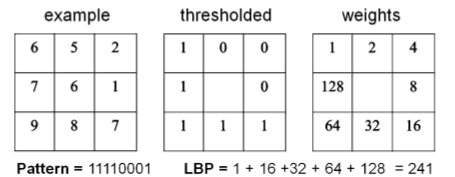
\includegraphics[scale=0.5]{lbp.png}
    \caption{LBP 3 x 3 (Pietik\"ainen, Hadid, Zhao \& Ahonen (2011))}
\end{figure}

The pattern will be an 8-bit integer. This is accomplished by shifting the
boolean value of each comparison one to seven places to the left.

This results in the following mathematical expression:

Let I($x_i, y_i$) be a grayscale Image and $g_n$ the value of the pixel $(x_i,
y_i)$. Also let $s(g_i, g_c)$ (see below) with $g_c$ being the value of the
center pixel and $g_i$ the grayscale value of the pixel to be evaluated.

$$
    s(g_i, g_c) = \left \{
    \begin{array}{l l}
        1 & \quad \text{if $g_i$ $\geq$ $g_c$}\\
        0 & \quad \text{if $g_i$ $<$ $g_c$}\\
    \end{array} \right.
$$

$$LBP_{n, g_c = (x_c, y_c)} = \sum\limits_{i=0}^{n-1} s(g_i, g_c) \cdot 2^i$$

The outcome of this operations will be a binary pattern. Note that the
mathematical expression has the same effect as the bit shifting operation that
we defined earlier.

\item Given this pattern for each pixel, the next step is to divide the image
into cells.

\item Compute a histogram for each cell.

\begin{figure}[H]
    \center
    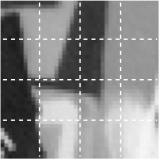
\includegraphics[scale=0.7]{cells.png}
    \caption{Divide into cells (Pietik\"ainen et all (2011))}
\end{figure}

\item Consider every histogram a vector element and concatenate all histograms.
The concatenation is the feature vector of the image.

\item Feed these vectors to a support vector machine. The SVM will ``learn''
which vectors to associate with a character.

\end{enumerate}

To our knowledge, LBP has yet not been used in this manner before. Therefore,
it will be the first thing to implement, to see if it lives up to the
expectations. When the proof of concept is there, it can be used in a final,
more efficient program.

Later we will show that taking a histogram over the entire image (basically
working with just one cell) gives us the best results.

\subsection{Matching the database}

Given the LBP of a character, a Support Vector Machine can be used to classify
the character to a character in a learning set. The SVM uses the concatenation
of the histograms of all cells in an image as a feature vector (in the case we
check the entire image no concatenation has to be done of course. The SVM can
be trained with a subset of the given dataset called the ``learning set''. Once
trained, the entire classifier can be saved as a Pickle object\footnote{See
\url{http://docs.python.org/library/pickle.html}} for later usage.
In our case the support vector machine uses a radial gauss kernel function. The
 SVM finds a seperating hyperplane with minimum margins.

\section{Implementation}

In this section we will describe our implementation in more detail, explaining
the choices we made in the process. We spent a lot of attention on structuring
the code in such a fashion that it can easily be extended.

\subsection{Character retrieval}

In order to retrieve the characters from the entire image, we need to
perform a perspective transformation. However, to do this, we need to know the
coordinates of the four corners of each character. For our dataset, this is
stored in XML files. So, the first step is to read these XML files.

\paragraph*{XML reader}

The XML reader will return a `license plate' object when given an XML file. The
licence plate holds a list of, up to six, NormalizedImage characters and from
which country the plate is from. The reader is currently assuming the XML file
and image name are corresponding, since this was the case for the given
dataset. This can easily be adjusted if required.

To parse the XML file, the minidom module is used. So the XML file can be
treated as a tree, where one can search for certain nodes. In each XML
file it is possible that multiple versions exist, so the first thing the reader
will do is retrieve the current and most up-to-date version of the plate. The
reader will only get results from this version.

Now we are only interested in the individual characters so we can skip the
location of the entire license plate. Each character has
a single character value, indicating what someone thought what the letter or
digit was and four coordinates to create a bounding box. If less then four
points have been set the character will not be saved. Else, to make things not
to complicated, a Character class is used. It acts as an associative list, but
it gives some extra freedom when using the data.

When four points have been gathered the data from the actual image is being
requested. For each corner a small margin is added (around 3 pixels) so that no
features will be lost and minimum amounts of new features will be introduced by
noise in the margin.

In the next section you can read more about the perspective transformation that
is being done. After the transformation the character can be saved: Converted
to grayscale, but nothing further. This was used to create a learning set. If
it does not need to be saved as an actual image it will be converted to a
NormalizedImage. When these actions have been completed for each character the
license plate is usable in the rest of the code.

\paragraph*{Perspective transformation}
Once we retrieved the corner points of the character, we feed those to a
module that extracts the (warped) character from the original image, and
creates a new image where the character is cut out, and is transformed to a
rectangle.

\subsection{Noise reduction}

The image contains a lot of noise, both from camera errors due to dark noise
etc., as from dirt on the license plate. In this case, noise therefore means
any unwanted difference in color from the surrounding pixels.

\paragraph*{Camera noise and small amounts of dirt}
The dirt on the license plate can be of different sizes. We can reduce the
smaller amounts of dirt in the same way as we reduce normal noise, by applying
a Gaussian blur to the image. This is the next step in our program.

The Gaussian filter we use comes from the \texttt{scipy.ndimage} module. We use
this function instead of our own function, because the standard functions are
most likely more optimized then our own implementation, and speed is an
important factor in this application.

\paragraph*{Larger amounts of dirt}
Larger amounts of dirt are not going to be resolved by using a Gaussian filter.
We rely on one of the characteristics of the Local Binary Pattern, only looking
at the difference between two pixels, to take care of these problems. \\
Because there will probably always be a difference between the characters and
the dirt, and the fact that the characters are very black, the shape of the
characters will still be conserved in the LBP, even if there is dirt
surrounding the character.

\subsection{Creating Local Binary Patterns and feature vector}
Every pixel is a center pixel and it is also a value to evaluate but not at the
same time. Every pixel is evaluated as shown in the explanation
of the LBP algorithm. There are several neighbourhoods we can evaluate. We have
tried the following neighbourhoods:

\begin{figure}[H]
    \center
    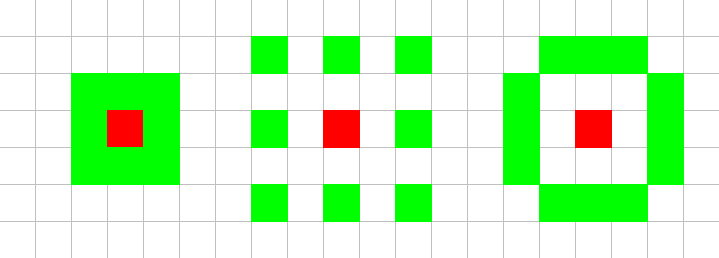
\includegraphics[scale=0.5]{neighbourhoods.png}
    \caption{Tested neighbourhoods}
    \label{fig:tested-neighbourhoods}
\end{figure}

We name these neighbourhoods respectively (8,3)-, (8,5)- and
(12,5)-neighbourhoods, after the number of points we use and the diameter
of the `circle´ on which these points lay.

We chose these neighbourhoods to prevent having to use interpolation, which
would add a computational step, thus making the code execute slower. In the
next section we will describe what the best neighbourhood was.

Take an example where the full square can be evaluated, so none of the
neighbours are out of bounds. The first to be checked is the pixel in the left
bottom corner in the square 3 x 3, with coordinate $(x - 1, y - 1)$ with $g_c$
as center pixel that has coordinates $(x, y)$. If the grayscale value of the
neighbour in the left corner is greater than the grayscale
value of the center pixel than return true. Bit-shift the first bit with 7. The
outcome is now 1000000. The second neighbour will be bit-shifted with 6, and so
on. Until we are at 0. The result is a binary pattern of the local point just
evaluated.
Now only the edge pixels are a problem, but a simple check if the location of
the neighbour is still in the image can resolve this. We simply state that the
pixel has a lower value then the center pixel if it is outside the image
bounds.

\paragraph*{Histogram and Feature Vector}
After all the Local Binary Patterns are created for every pixel, this pattern
is divided into cells. The feature vector is the vector of concatenated
histograms. These histograms are created for cells. These cells are created by
dividing the \textbf{pattern} in to cells and create a histogram of that. So
multiple cells are related to one histogram. All the histograms are
concatenated and fed to the SVM that will be discussed in the next section,
Classification. We did however find out that the use of several cells was not
increasing our performance, so we only have one histogram to feed to the SVM.

\subsection{Classification}

For the classification, we use a standard Python Support Vector Machine,
\texttt{libsvm}. This is an often used SVM, and should allow us to simply feed
data from the LBP and Feature Vector steps into the SVM and receive results.



Usage a SVM can be divided in two steps. First, the SVM has to be trained
before it can be used to classify data. The training step takes a lot of time,
but luckily \texttt{libsvm} offers us an opportunity to save a trained SVM.
This means that the SVM only has to be created once, and can be saved for later
usage.

We have decided only to include a character in the system if the SVM can be
trained with 70 examples. This is done automatically, by splitting the data set
in a learning set and a test set, where the first 70 occurrences of a character
are added to the learning set, and all the following are added to the test set.
Therefore, if there are not enough examples, all available occurrences end up
in the learning set, and non of these characters end up in the test set. Thus,
they do not decrease our score. If such a character would be offered to the
system (which it will not be in out own test program), the SVM will recognize
it as good as possible because all occurrences are in the learning set.

\subsection{Supporting Scripts}

To be able to use the code efficiently, we wrote a number of scripts. This
section describes the purpose and usage of each script.

\subsection*{\texttt{create\_characters.py}}



\subsection*{\texttt{create\_classifier.py}}



\subsection*{\texttt{find\_svm\_params.py}}



\subsection*{\texttt{generate\_learning\_set.py}}



\subsection*{\texttt{load\_learning\_set.py}}



\subsection*{\texttt{run\_classifier.py}}



\section{Finding parameters}

Now that we have a functioning system, we need to tune it to work properly for
license plates. This means we need to find the parameters. Throughout the
program we have a number of parameters for which no standard choice is
available. These parameters are:

\begin{tabular}{l|l}
	Parameter 			& Description \\
	\hline
	$\sigma$  			& The size of the Gaussian blur. \\
	\emph{cell size}	& The size of a cell for which a histogram of LBP's
	                      will be generated. \\
	\emph{Neighbourhood}& The neighbourhood to use for creating the LBP. \\
	$\gamma$			& Parameter for the Radial kernel used in the SVM. \\
	$c$					& The soft margin of the SVM. Allows how much training
						  errors are accepted. \\
\end{tabular}

For each of these parameters, we will describe how we searched for a good
value, and what value we decided on.

\subsection{Parameter $\sigma$}

The first parameter to decide on, is the $\sigma$ used in the Gaussian blur. To
find this parameter, we tested a few values, by trying them and checking the
results. It turned out that the best value was $\sigma = 1.4$.

Theoretically, this can be explained as follows. The filter has width of
$6 * \sigma = 6 * 1.4 = 8.4$ pixels. The width of a `stroke' in a character is,
after our resize operations, around 8 pixels. This means, our filter `matches'
the smallest detail size we want to be able to see, so everything that is
smaller is properly suppressed, yet it retains the details we do want to keep,
being everything that is part of the character.

\subsection{Parameter \emph{cell size}}

The cell size of the Local Binary Patterns determines over what region a
histogram is made. The trade-off here is that a bigger cell size makes the
classification less affected by relative movement of a character compared to
those in the learning set, since the important structure will be more likely to
remain in the same cell. However, if the cell size is too big, there will not
be enough cells to properly describe the different areas of the character, and
the feature vectors will not have enough elements.

In order to find this parameter, we used a trial-and-error technique on a few
cell sizes. During this testing, we discovered that a lot better score was
reached when we take the histogram over the entire image, so with a single
cell. Therefore, we decided to work without cells.

A reason we can think of why using one cell works best is that the size of a
single character on a license plate in the provided dataset is very small.
That means that when dividing it into cells, these cells become simply too
small to have a really representative histogram. Therefore, the
concatenated histograms are then a list of only very small numbers, which
are not significant enough to allow for reliable classification.

\subsection{Parameter \emph{Neighbourhood}}

We tested the classifier with the patterns given in figure
\ref{fig:tested-neighbourhoods}. We found that the best results were reached
with the following neighbourhood, which we will call the (12,5)-neighbourhood,
since it has 12 points in a area with a diameter of 5.

\begin{figure}[H]
    \center
    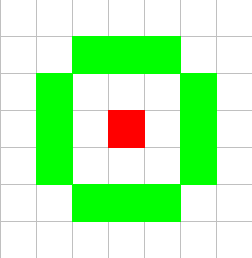
\includegraphics[scale=0.5]{12-5neighbourhood.png}
    \caption{(12,5)-neighbourhood}
\end{figure}

\subsection{Parameters $\gamma$ \& $c$}

The parameters $\gamma$ and $c$ are used for the SVM. $c$ is a standard
parameter for each type of SVM, called the `soft margin'. This determines the
amount of overlap that is allowed between two SVM-classes (which, in this case,
are characters). Below, we will illustrate that the optimal value for $c$ is
32, which means that there is an overlap between classes. This can be explained
by the fact that some characters are very similar to eachother. For instance, a
`Z' is similar to a `7' and a `B' is similar to an `R'.

$\gamma$ is a variable that determines the shape of the radial kernel, and as
such determines how strongly the vector space of the SVM is transformed by the
kernel function.

To find the optimal combination of values for these variables, we have
performed a so-called grid-search. A grid-search takes exponentially growing
sequences for each parameter, and tests a classifier for each combination of
values. The combination with the highest score is the optimal solution, which
will be used in the final classifier.

The results of our grid-search are displayed in the following table. The values
in the table are rounded percentages, for better readability.

\begin{tabular}{|r|r r r r r r r r r r|}
\hline
c $\gamma$ & $2^{-15}$ & $2^{-13}$ & $2^{-11}$ & $2^{-9}$ & $2^{-7}$ &
	$2^{-5}$ & $2^{-3}$ & $2^{-1}$ & $2^{1}$ & $2^{3}$\\
\hline
$2^{-5}$ &       61 &       61 &       61 &       61 &       62 &
       63 &       67 &       74 &       59 &       24\\
$2^{-3}$ &       61 &       61 &       61 &       61 &       62 &
       63 &       70 &       78 &       60 &       24\\
$2^{-1}$ &       61 &       61 &       61 &       61 &       62 &
       70 &       83 &       88 &       78 &       27\\
 $2^{1}$ &       61 &       61 &       61 &       61 &       70 &
        84 &       90 &       92 &       86 &       45\\
 $2^{3}$ &       61 &       61 &       61 &       70 &       84 &
        90 &       93 &       93 &       86 &       45\\
 $2^{5}$ &       61 &       61 &       70 &       84 &       90 &
        92 &       93 &       93 &       86 &       45\\
 $2^{7}$ &       61 &       70 &       84 &       90 &       92 &
        93 &       93 &       93 &       86 &       45\\
 $2^{9}$ &       70 &       84 &       90 &       92 &       92 &
       93 &       93 &       93 &       86 &       45\\
$2^{11}$ &       84 &       90 &       92 &       92 &       92 &
       92 &       93 &       93 &       86 &       45\\
$2^{13}$ &       90 &       92 &       92 &       92 &       92 &
       92 &       93 &       93 &       86 &       45\\
$2^{15}$ &       92 &       92 &       92 &       92 &       92 &
       92 &       93 &       93 &       86 &       45\\
\hline
\end{tabular} \\

The grid-search shows that the best values for these parameters are $c = 2^5 =
32$ and $\gamma = 2^{-3} = 0.125$.

\section{Results}

\subsection{Accuracy}

The main goal of this project is to find out if LBP is a suitable algorithm to
classify license plate characters.

Of course, it is vital that the recognition of a license plate is correct,
almost correct is not good enough here. Therefore, the highest possible score
must be reached.

According to Wikipedia \cite{wikiplate}, commercial license plate recognition
that are currently on the market software score about $90\%$ to $94\%$, under
optimal conditions and with modern equipment.

Our program scores an average of $93\%$. However, this is for a single
character. That means that a full license plate should theoretically
get a score of $0.93^6 = 0.647$, so $64.7\%$. That is not particularly
good compared to the commercial ones. However, our focus was on getting
good scores per character. For us, $93\%$ is a very satisfying result.

Possibilities for improvement of this score would be more extensive
grid-searches, finding more exact values for $c$ and $\gamma$, more tests
for finding $\sigma$ and more experiments on the size and shape of the
neighbourhoods.

\subsubsection*{Faulty classified characters}

As we do not have a $100\%$ score, it is interesting to see what characters are
classified wrong. These characters are shown in appendix \ref{fcc}. Most of
these errors are easily explained. For example, some 0's are classified as
'D', some 1's are classified as 'T' and some 'F's are classified as 'E'.

Of course, these are not as interesting as some of the weird matches. For
example, a 'P' is classified as 7. However, if we look more closely, the 'P' is
standing diagonal, possibly because the datapoints where not very exact in the
XML file. This creates a large diagonal line in the image, which explains why
this can be classified as a 7. The same has happened with a 'T', which is also
marked as 7.

Other strange matches include a 'Z' as a 9, but this character has a lot of
noise surrounding it, which makes classification harder, and a 3 that is
classified as 9, where the exact opposite is the case. This plate has no noise,
due to which the background is a large area of equal color. This might cause
the classification to focus more on this than on the actual character.

\subsection{Speed}

Recognizing license plates is something that has to be done fast, since there
can be a lot of cars passing a camera in a short time, especially on a highway.
Therefore, we measured how well our program performed in terms of speed. We
measure the time used to normalize a character, create its feature vector and
classify it using a given classifier. The time needed to train the classifier
needs not to be measured, because that can be done `offline'.

We ran performance tests for the (8,3)- and (12,5)-patterns, with Gaussian blur
scales of $1.0$ and $1.4$ respectively on the same set of characters. Because
$1.5$ times an many pixel comparisons have to be executed (12 vs. 8), we
suspected an increase of at least $0.5$ times the time for the first test to be
the outcome of the second test. `At least', because the classification step
will also be slower due to the increased size of the feature vectors
($\frac{2^{12}}{2^8} = 2^4 = 16$ times as slow). The tests resulted in $81ms$
and $137ms$ per character. $\frac{137}{81} = 1.7$, which agrees with our
expectations. \\
Note: Both tests were executed using an AMD Phenom II X4 955 CPU processor,
running at 3.2 GHz.

This is not spectacular considering the amount of calculating power this CPU
can offer, but it is still fairly reasonable. Of course, this program is
written in Python, and is therefore not nearly as optimized as would be
possible when written in a low-level language.

Another performance gain is by using one of the other two neighbourhoods.
Since these have 8 points instead of 12 points, this increases performance
drastically, but at the cost of accuracy. With the (8,5)-neighbourhood
we only need 81ms seconds to identify a character. However, the accuracy
drops to $89\%$. When using the (8,3)-neighbourhood, the speedwise performance
remains the same, but accuracy drops even further, so that neighbourhood
is not advisable to use.

\section{Discussion}

There are a few points open for improvement. These are the following.

\subsection{Other Local Binary Patterns}

We had some good results but of course there are more things to explore.
For instance we did a research on three different patterns. There are more
patterns to try. For instance we only tried (8,3)-, (8,5)- and
(12,5)-neighbourhoods. What might be done is to test which pattern gives the
best result, for a wider range of neighbourhoods. We haven proven that the size
and number of points do influence the performance of the classifier, so further
research would be in place.

The expectation is that using a larger diameter pattern, but with the same
amount of points is worth trying. The theory behind that is that when using a
Gaussian blur to reduce noise, the edges are blurred as well. By taking larger
radius, you look over a larger distance, so the blurry part of the edge is
skipped. By not using more points, there is no penalty in the time needed to
calculate this larger pattern, so there is an accuracy advantage `for free'.

\subsection{Context Information}

We don't do assumption when a letter is recognized. For instance Dutch licence
plates exist of three blocks, two digits or two characters. Or for the new
licence plates there are three blocks, two digits followed by three characters,
followed by one or two digits. The assumption we can do is when there is have a
case when one digit is most likely to follow by a second digit and not a
character. Maybe these assumption can help in future research to achieve a
higher accuracy rate.

\subsection{Speed up}

A possibility to improve the performance speedwise would be to separate the
creation of the Gaussian kernel and the convolution. This way, the kernel can
be cached, which is a big improvement. At this moment, we calculate this kernel
every time a blur is applied to a character. This was done so we could use a
standard Python function, but we realised too late that there is performance
loss due to this.

Another performance loss was introduced by checking for each pixel if it is
in the image. This induces one function call and four conditional checks
per pixel, which costs performance. A faster method would be to first set a
border of black pixels around the image, so the inImage function is now done
implicitly because it simply finds a black pixel if it falls outside the
original image borders.

\section{Conclusion}

In the end it turns out that using Local Binary Patterns is a promising
technique for License Plate Recognition. It seems to be relatively indifferent
for the amount of dirt on license plates and different fonts on these plates.

The performance speed wise is fairly good, when using a fast machine. However,
this is written in Python, which means it is not as efficient as it could be
when using a low-level languages.

We believe that with further experimentation and development, LBP's can
absolutely be used as a good license plate recognition method.

\section{Reflection}

\subsection{Difficulties}

During the implementation and testing of the program, we did encounter a
number of difficulties. In this section we will state what these difficulties
were and whether we were able to find a proper solution for them.

\subsubsection*{Dataset}

We did experience a number of problems with the provided dataset. A number of
these are problems to be expected in a real world problem, but which make
development harder. Others are more elemental problems.

The first problem was that the dataset contains a lot of license plates which
are problematic to read, due to excessive amounts of dirt on them. Of course,
this is something you would encounter in the real situation, but it made it
hard for us to see whether there was a coding error or just a bad example.
aucla
Another problem was that there were license plates of several countries in
the dataset. Each of these countries has it own font, which also makes it
hard to identify these plates, unless there are a lot of these plates in the
learning set.

A problem that is more elemental is that some of the characters in the dataset
are not properly classified. This is of course very problematic, both for
training the SVM as for checking the performance. This meant we had to check
each character whether its description was correct.

As final note, we would like to state that an, in our eyes, unrealistic amount
of characters has a bad quality, with a lot of dirt, or crooked plates
etcetera. Our own experience is that the average license plate is less hard to
read. The local binary pattern method has proven to work on this set, and as
such has proven that it performs good in worst-case scenarios, but we would
like to see how it performs on a more realistic dataset.

\subsubsection*{SVM}

We also had trouble with the SVM for Python. The standard Python SVM, libsvm,
had a poor documentation. There was no explanation what so ever on which
parameter had to be what. This made it a lot harder for us to see what went
wrong in the program.

\subsection{Workload distribution}

The first two weeks were team based. Basically the LBP algorithm could be
implemented in the first hour, while some talked and someone did the typing.
Some additional 'basics' where created in similar fashion. This ensured that
every team member was up-to-date and could start figuring out which part of the
implementation was most suited to be done by one individually or in a pair.

\subsubsection*{Work distribution}

Gijs created the basic classes we could use and helped everyone by keeping
track of what was required to be finished and whom was working on what.
Gijs also worked with Tadde\"us on the Local Binary Patterns code.
Tadde\"us and Jayke worked on the SVM and Tadde\"us wrote all kinds of tests
for testing what part went good and what went wrong, and what parameters had
to be used. Fabi\"en created the functions to read and parse the given XML
files with information about the license plates. Upon completion all kinds
of learning and data sets could be created. Richard helped out wherever
anyone needed a helping hand, and was always available when someone had
doubts about what they where doing or needed to ask something. He also wrote
an image cropper that exactly cuts out a character, which eventually turned
out to be obsolete. The work on the report was mainly done by Jayke, assisted
by Fabi\"en and Richard and the technical details were filled in by Gijs and
Tadde\"us.

\appendix

\section{Faulty classified characters}
\label{fcc}

\begin{figure}[H]
    \hspace{-2cm}
    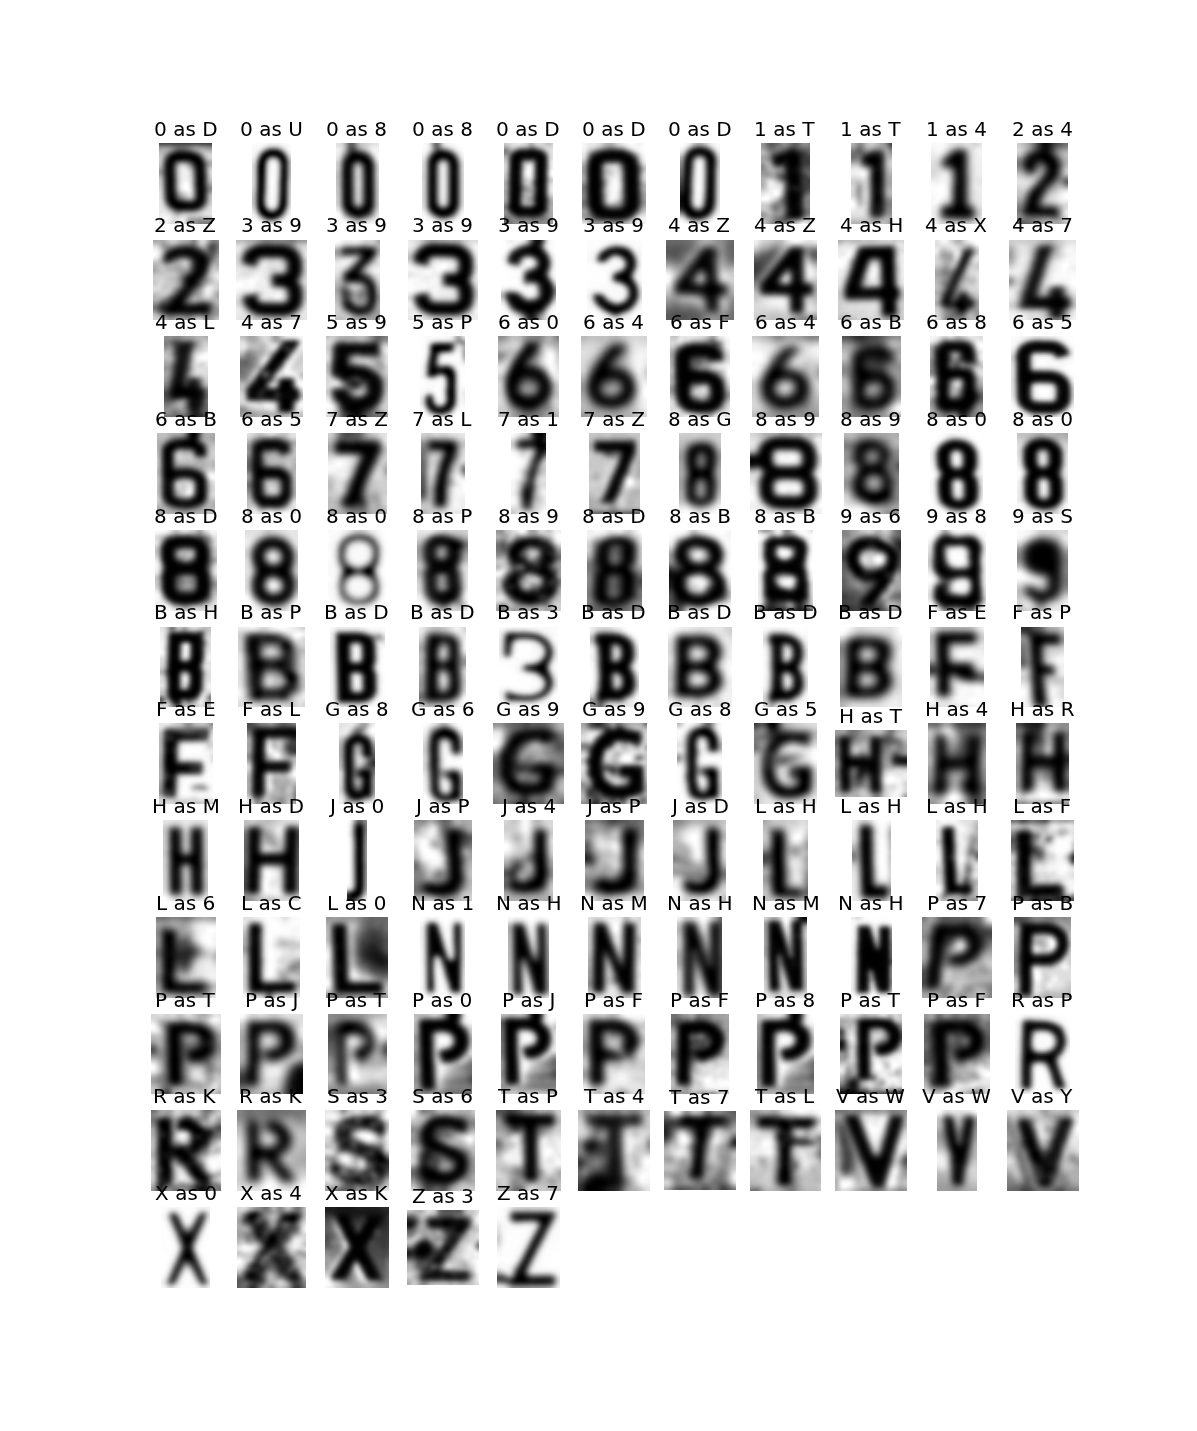
\includegraphics[scale=0.5]{faulty.png}
    \caption{Faulty classificatied characters}
\end{figure}

\begin{thebibliography}{9}
    \bibitem{lbp1}
        Matti Pietik\"ainen, Guoyin Zhao, Abdenour hadid,
        Timo Ahonen.
        \emph{Computational Imaging and Vision}.
        Springer-Verlag, London,
        1st Edition,
        2011.
    \bibitem{wikiplate}
        \emph{Automatic number-plate recognition}. (2011, December 17). \\
        Wikipedia.
        Retrieved from
        \url{http://en.wikipedia.org/wiki/Automatic_number_plate_recognitiona}
\end{thebibliography}

\end{document}
